\chapter{Introduction} \label{ch:introduction}

The FDTD \cite{Yee} algorithm is the underlying mechanism used by many commercial RF simulation packages, as well as open source software such as MIT's Meep. 

Given the computationally-intensive nature of FDTD, organizations requiring simulation of large domains or complex circuits must provide significant resources. These may take the form of leased server time or utilization of an on-site high-performance cluster, amongst other options.

In this thesis, we explore an implementation of FDTD utilizing graphics processing units (GPUs). Initially designed to perform image generation tasks such as those required by games, cinema and related fields, modern versions are well-suited for general computation work. GPUs are now enjoying wide adoption in fields such as machine learning and artificial intelligence, medical research, signals analysis and other areas which require rapid analysis of large datasets.

Even modern consumer-grade GPUs offer thousands or tens of thousands of processing units ("cores"), while high-end CPUs typically offer 4-8 cores. While the two are not interchangeable, some algorithms, such as FDTD, require little or no data interdependence, no branching logic (a severe performance impediment on GPUs) and consist of short cycles of simple operations. The power of the GPU lies in performing these simple operations at large scale, with thousands of threads running in parallel. 

The following sections detail FDTD. Later sections describe a CPU-based implementation (MIT's  Meep simulator), and our GPU-based GoLightly simulator. We verify the GPU solution numerically, and compare performance between CPU- and GPU-based implementations. Finally, we consider future applications and enhancements. 


\section{FDTD Overview}

At it's heart, FDTD expresses Maxwell's equations as a discretized set of time-domain equations. These equations describe each electric field component in terms if its orthogonal, coupled magnetic fields, and each magnetic field component as a function of its coupled, orthogonal electric fields.


\subsection{Wave equation}

In a $TM_z$ time domain simulation, wave equation for  $ E_z $ is of the form:

\begin{equation} \label{eq:waveequation} 
\frac{\partial E_z}{\partial t} = K * (\frac{\partial H_x}{\partial y} + \frac{\partial H_y}{\partial x})
\end{equation}

Equation \ref{eq:waveequation} states that the temporal derivative (change in amplitude) of $E_z$ is a function of the $Y$-axis spatial derivative of the $H_x$ field and the $X$-axis spatial derivative of the $H_y$ field.


In order to apply this equation to a computational domain, FDTD defines a cell-based discretization strategy.

\subsection{Yee Cell}

Yee \cite{Yee} defines a computational unit known as a "cell." The cell describes how each field component within a domain is related to it's coupled fields. For instance, in a 2D $TM_z$ simulation, $E_Z$ depends on adjacent $H_y$ and $H_x$ components. The cell format used in such a simulation is of the form shown in \ref{fig:yeecell}.

\begin{figure}[H]
	\centering
	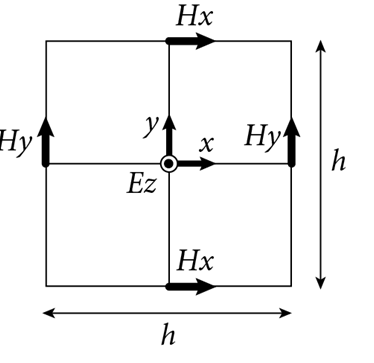
\includegraphics{yee-cell-ez.png}
	\caption{2D $TM_Z$ Yee Cell}
	\label{fig:yeecell}
\end{figure}

More formally, we may expand the $E_Z$ wave equation, arriving at:

\begin{equation} \label{eq:ezupdate}
{E_z}_{i,j}^{t} = C_a * {E_z}_{i,j}^{t-1} 
+ C_b * ({H_x}_{i,j+\frac{1}{2}}^{t-\frac{1}{2}} - {H_x}_{i,j-\frac{1}{2}}^{t-\frac{1}{2}})
+ C_b * ({H_y}_{i+\frac{1}{2},j}^{t-\frac{1}{2}} - {H_xy}_{i-\frac{1}{2},j}^{t-\frac{1}{2}})
\end{equation}

Similarly, the equations for the coupled fields $H_x$ and $H_y$ may be expressed as:
\begin{equation} \label{eq:hxupdate}
{H_x}_{i,j}^t = D_a * {H_x}_{i,j}^{t-1} + D_b * (
{E_z}_{i,j+\frac{1}{2}}^{t-\frac{1}{2}} 
-
{E_z}_{i,j-\frac{1}{2}}^{t-\frac{1}{2}}
)  
\end{equation}

\begin{equation} \label{eq:hyupdate}
{H_y}_{i,j}^t = D_a * {H_y}_{i,j}^{t-1} + D_b * (
{E_z}_{i+\frac{1}{2},j}^{t-\frac{1}{2}} 
-
{E_z}_{i-\frac{1}{2},j}^{t-\frac{1}{2}}
)  
\end{equation}


%\begin{table}[ht]
%	\caption{FDTD Coefficients}
%	\centering
%	\begin{tabular}{c c c}
%		\hline\hline
%		Symbol & Value & Meaning \\
%		\hline
%		$C_a$ & & \\
%		$C_b$ & & \\
%		$D_a$ & & \\
%		$D_b$ & & \\
%		\hline
%	\end{tabular}
%	\label{table:fdtdcoefficients}
%\end{table}











